\section{Notation}
In this section we will briefly explain the mathematical notation and model used in the paper. The graph representation consists of edges which represents roads and vertices which represents either charge stations or road intersections. We define a \textbf{road network} as an ordered pair \(G=(V,E)\) comprising of a set $V$ of vertices together with a set $E$ of edges. Where $V$ is a finite set and $E$ is a binary relation on $V$. We further define the following functions:
\[ E_d(u,v)\rightarrow d \] 
\[ E_v(u,v)\rightarrow v \] 
These are partial functions defined by the edge $(u,v)$ and respectively returns a distance or a speed limit.

Each vertex is then defined as a \textit{charge station}, described by the following partial function:
\[V_c(v)\rightarrow c\]
A road intersection is simply a vertex with charge rate $c = 0$, while a charge station is a vertex where $c > 0$. An electrical vehicle is specified by two parameters: It's battery capacity ($kWh$), consumption rate ($kWh/km$). The consumption rate is given by the following function:

\[C_R(v)=av^2+bv+c\]
% \[ 4,60272*10^{-5}*v^2+6,59187*10^{-4}*v+0,173117 \] tesla

where $v$ is the speed of the vehicle. 

\begin{figure}
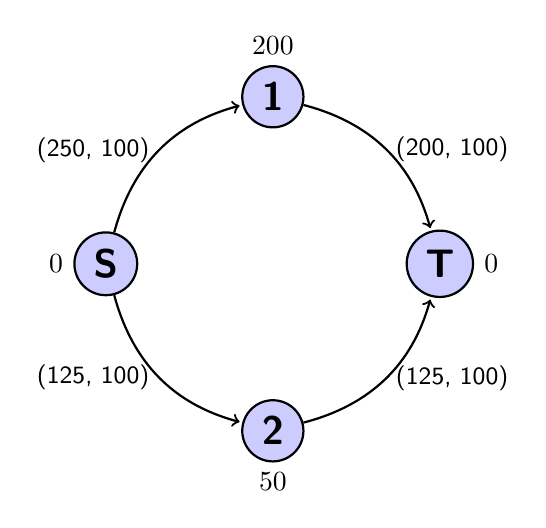
\begin{tikzpicture}[->,->,shorten >=1pt,auto,node distance=3cm,
  thick,main node/.style={circle,fill=blue!20,draw,font=\sffamily\Large\bfseries}]
%1
  \node[main node] (1) {1};
  \node[above] at (1.north) {200};
%2 
 \node[main node] (2) [below left of=1] {S};
  \node[left] at (2.west) {0};
%3 
 \node[main node] (3) [below right of=2] {2};
  \node[below] at (3.south) {50};
%4 
 \node[main node] (4) [below right of=1] {T};
  \node[right] at (4.east) {0};
%paths
  \path[every node/.style={font=\sffamily\small}]
    (1)
	  edge [bend left] node[right] {(200, 100)} (4)
    (2) edge [bend right] node[left] {(125, 100)} (3)
    	  edge [bend left] node[left] {(250, 100)} (1)
    (3) edge [bend right] node[right] {(125, 100)} (4)
    (4) ;
\end{tikzpicture}

\label{figure:simpleroad-network}
\caption{A simple road-network with starting point s and end point t}
\end{figure}

\todo[inline]{Add notation about path, more about vehicle and maybe describe a solution}
